% Options for packages loaded elsewhere
\PassOptionsToPackage{unicode}{hyperref}
\PassOptionsToPackage{hyphens}{url}
\PassOptionsToPackage{dvipsnames,svgnames,x11names}{xcolor}
%
\documentclass[
  letterpaper,
  DIV=11,
  numbers=noendperiod]{scrartcl}

\usepackage{amsmath,amssymb}
\usepackage{lmodern}
\usepackage{iftex}
\ifPDFTeX
  \usepackage[T1]{fontenc}
  \usepackage[utf8]{inputenc}
  \usepackage{textcomp} % provide euro and other symbols
\else % if luatex or xetex
  \usepackage{unicode-math}
  \defaultfontfeatures{Scale=MatchLowercase}
  \defaultfontfeatures[\rmfamily]{Ligatures=TeX,Scale=1}
  \setmainfont[]{DejaVu Sans}
\fi
% Use upquote if available, for straight quotes in verbatim environments
\IfFileExists{upquote.sty}{\usepackage{upquote}}{}
\IfFileExists{microtype.sty}{% use microtype if available
  \usepackage[]{microtype}
  \UseMicrotypeSet[protrusion]{basicmath} % disable protrusion for tt fonts
}{}
\makeatletter
\@ifundefined{KOMAClassName}{% if non-KOMA class
  \IfFileExists{parskip.sty}{%
    \usepackage{parskip}
  }{% else
    \setlength{\parindent}{0pt}
    \setlength{\parskip}{6pt plus 2pt minus 1pt}}
}{% if KOMA class
  \KOMAoptions{parskip=half}}
\makeatother
\usepackage{xcolor}
\setlength{\emergencystretch}{3em} % prevent overfull lines
\setcounter{secnumdepth}{5}
% Make \paragraph and \subparagraph free-standing
\ifx\paragraph\undefined\else
  \let\oldparagraph\paragraph
  \renewcommand{\paragraph}[1]{\oldparagraph{#1}\mbox{}}
\fi
\ifx\subparagraph\undefined\else
  \let\oldsubparagraph\subparagraph
  \renewcommand{\subparagraph}[1]{\oldsubparagraph{#1}\mbox{}}
\fi


\providecommand{\tightlist}{%
  \setlength{\itemsep}{0pt}\setlength{\parskip}{0pt}}\usepackage{longtable,booktabs,array}
\usepackage{calc} % for calculating minipage widths
% Correct order of tables after \paragraph or \subparagraph
\usepackage{etoolbox}
\makeatletter
\patchcmd\longtable{\par}{\if@noskipsec\mbox{}\fi\par}{}{}
\makeatother
% Allow footnotes in longtable head/foot
\IfFileExists{footnotehyper.sty}{\usepackage{footnotehyper}}{\usepackage{footnote}}
\makesavenoteenv{longtable}
\usepackage{graphicx}
\makeatletter
\def\maxwidth{\ifdim\Gin@nat@width>\linewidth\linewidth\else\Gin@nat@width\fi}
\def\maxheight{\ifdim\Gin@nat@height>\textheight\textheight\else\Gin@nat@height\fi}
\makeatother
% Scale images if necessary, so that they will not overflow the page
% margins by default, and it is still possible to overwrite the defaults
% using explicit options in \includegraphics[width, height, ...]{}
\setkeys{Gin}{width=\maxwidth,height=\maxheight,keepaspectratio}
% Set default figure placement to htbp
\makeatletter
\def\fps@figure{htbp}
\makeatother

\KOMAoption{captions}{tableheading}
\makeatletter
\@ifpackageloaded{tcolorbox}{}{\usepackage[many]{tcolorbox}}
\@ifpackageloaded{fontawesome5}{}{\usepackage{fontawesome5}}
\definecolor{quarto-callout-color}{HTML}{909090}
\definecolor{quarto-callout-note-color}{HTML}{0758E5}
\definecolor{quarto-callout-important-color}{HTML}{CC1914}
\definecolor{quarto-callout-warning-color}{HTML}{EB9113}
\definecolor{quarto-callout-tip-color}{HTML}{00A047}
\definecolor{quarto-callout-caution-color}{HTML}{FC5300}
\definecolor{quarto-callout-color-frame}{HTML}{acacac}
\definecolor{quarto-callout-note-color-frame}{HTML}{4582ec}
\definecolor{quarto-callout-important-color-frame}{HTML}{d9534f}
\definecolor{quarto-callout-warning-color-frame}{HTML}{f0ad4e}
\definecolor{quarto-callout-tip-color-frame}{HTML}{02b875}
\definecolor{quarto-callout-caution-color-frame}{HTML}{fd7e14}
\makeatother
\makeatletter
\makeatother
\makeatletter
\makeatother
\makeatletter
\@ifpackageloaded{caption}{}{\usepackage{caption}}
\AtBeginDocument{%
\ifdefined\contentsname
  \renewcommand*\contentsname{Table of contents}
\else
  \newcommand\contentsname{Table of contents}
\fi
\ifdefined\listfigurename
  \renewcommand*\listfigurename{List of Figures}
\else
  \newcommand\listfigurename{List of Figures}
\fi
\ifdefined\listtablename
  \renewcommand*\listtablename{List of Tables}
\else
  \newcommand\listtablename{List of Tables}
\fi
\ifdefined\figurename
  \renewcommand*\figurename{Figure}
\else
  \newcommand\figurename{Figure}
\fi
\ifdefined\tablename
  \renewcommand*\tablename{Table}
\else
  \newcommand\tablename{Table}
\fi
}
\@ifpackageloaded{float}{}{\usepackage{float}}
\floatstyle{ruled}
\@ifundefined{c@chapter}{\newfloat{codelisting}{h}{lop}}{\newfloat{codelisting}{h}{lop}[chapter]}
\floatname{codelisting}{Listing}
\newcommand*\listoflistings{\listof{codelisting}{List of Listings}}
\makeatother
\makeatletter
\@ifpackageloaded{caption}{}{\usepackage{caption}}
\@ifpackageloaded{subcaption}{}{\usepackage{subcaption}}
\makeatother
\makeatletter
\@ifpackageloaded{tcolorbox}{}{\usepackage[many]{tcolorbox}}
\makeatother
\makeatletter
\@ifundefined{shadecolor}{\definecolor{shadecolor}{rgb}{.97, .97, .97}}
\makeatother
\makeatletter
\makeatother
\ifLuaTeX
  \usepackage{selnolig}  % disable illegal ligatures
\fi
\IfFileExists{bookmark.sty}{\usepackage{bookmark}}{\usepackage{hyperref}}
\IfFileExists{xurl.sty}{\usepackage{xurl}}{} % add URL line breaks if available
\urlstyle{same} % disable monospaced font for URLs
\hypersetup{
  pdftitle={Data Science for Public Health workshop},
  colorlinks=true,
  linkcolor={blue},
  filecolor={Maroon},
  citecolor={Blue},
  urlcolor={Blue},
  pdfcreator={LaTeX via pandoc}}

\title{Data Science for Public Health workshop}
\usepackage{etoolbox}
\makeatletter
\providecommand{\subtitle}[1]{% add subtitle to \maketitle
  \apptocmd{\@title}{\par {\large #1 \par}}{}{}
}
\makeatother
\subtitle{Information}
\author{}
\date{}

\begin{document}
\maketitle
\ifdefined\Shaded\renewenvironment{Shaded}{\begin{tcolorbox}[sharp corners, frame hidden, breakable, interior hidden, enhanced, boxrule=0pt, borderline west={3pt}{0pt}{shadecolor}]}{\end{tcolorbox}}\fi

\begin{longtable}[]{@{}l@{}}
\toprule()
\endhead
September 26-28, 2022 \\
09:00 - 17:00 \\
Dar-es-Salaam, Tanzania \\
\bottomrule()
\end{longtable}

This workshop targets public health researchers and aims to accompany
them in their journey towards Data Science. Looking forward to meeting
you all on Monday!

\hypertarget{venue}{%
\section{Venue}\label{venue}}

The workshop takes place at \textbf{Protea Hotel Dar es Salaam
Courtyard} on Seaview Ocean Road. The conference room is \textbf{Nelson
Hall}.

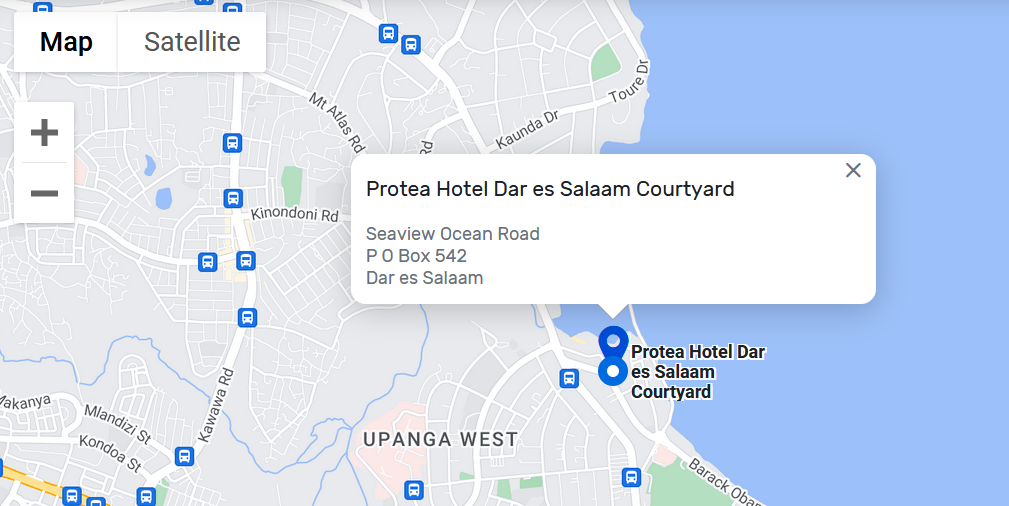
\includegraphics{images/paste-67B4C38F.png}

\hypertarget{before-the-workshop}{%
\section{Before the workshop}\label{before-the-workshop}}

\begin{enumerate}
\def\labelenumi{\arabic{enumi}.}
\item
  Fill out the online
  \href{https://timicodktest.smartforest.de/-/single/cac06e76b3e163e655e49626f8129de8f55a8035ced54f15bc4c6cf527dba8a7?st=DnBRz677PIYh33ML0rE1amWzyhCIYPGFQnmZ6AAou8nJFyikWN6nLM5i3G4I0YZN}{pre-workshop
  questionnaire}
\item
  If you have not done it yet, please go through the following five
  steps (about 30 minutes).

  \begin{enumerate}
  \def\labelenumii{\alph{enumii}.}
  \item
    \href{https://thaliehln.github.io/ds4ph/r_setup.html\#sec-R-installation}{Install
    R}
  \item
    \href{https://thaliehln.github.io/ds4ph/r_setup.html\#sec-RStudio-installation}{Install
    and setup RStudio Desktop}
  \item
    \href{https://thaliehln.github.io/ds4ph/r_setup.html\#sec-Quarto-installation}{Install
    Quarto}
  \item
    \href{https://thaliehln.github.io/ds4ph/r_setup.html\#sec-rmarkdown-installation}{Install
    the rmarkdown R package}
  \item
    \href{https://thaliehln.github.io/ds4ph/github_setup.html\#sec-GitHub-account-creation}{Create
    a GitHub account}
  \item
    \href{https://thaliehln.github.io/ds4ph/github_setup.html\#sec-GitHub-Desktop-installation}{Install
    GitHub Desktop}
  \end{enumerate}
\end{enumerate}

\begin{tcolorbox}[enhanced jigsaw, coltitle=black, bottomrule=.15mm, toptitle=1mm, colframe=quarto-callout-note-color-frame, colback=white, bottomtitle=1mm, rightrule=.15mm, opacityback=0, breakable, leftrule=.75mm, opacitybacktitle=0.6, left=2mm, titlerule=0mm, toprule=.15mm, title=\textcolor{quarto-callout-note-color}{\faInfo}\hspace{0.5em}{Note}, arc=.35mm, colbacktitle=quarto-callout-note-color!10!white]

\begin{itemize}
\tightlist
\item
  All software used in this workshop are free.
\item
  If you have any difficulties with the installation, support can be
  provided on the first day of the workshop before the first session or
  during breaks.
\end{itemize}

\end{tcolorbox}

\begin{tcolorbox}[enhanced jigsaw, coltitle=black, bottomrule=.15mm, toptitle=1mm, colframe=quarto-callout-important-color-frame, colback=white, bottomtitle=1mm, rightrule=.15mm, opacityback=0, breakable, leftrule=.75mm, opacitybacktitle=0.6, left=2mm, titlerule=0mm, toprule=.15mm, title=\textcolor{quarto-callout-important-color}{\faExclamation}\hspace{0.5em}{Important}, arc=.35mm, colbacktitle=quarto-callout-important-color!10!white]
For those who have already been introduced to Git, R/RStudio and
RMarkdown, note that you need to additionally install Quarto for this
workshop.
\end{tcolorbox}

\newpage{}

\hypertarget{schedule}{%
\section{Schedule}\label{schedule}}

\hypertarget{day-1-monday-september-26th}{%
\subsection{Day 1: Monday September
26th}\label{day-1-monday-september-26th}}

\hypertarget{tbl-day1-schedule}{}
\begin{longtable}[]{@{}
  >{\centering\arraybackslash}p{(\columnwidth - 2\tabcolsep) * \real{0.2361}}
  >{\raggedright\arraybackslash}p{(\columnwidth - 2\tabcolsep) * \real{0.6528}}@{}}
\caption{\label{tbl-day1-schedule}Overview Day 1}\tabularnewline
\toprule()
\begin{minipage}[b]{\linewidth}\centering
Time
\end{minipage} & \begin{minipage}[b]{\linewidth}\raggedright
Session
\end{minipage} \\
\midrule()
\endfirsthead
\toprule()
\begin{minipage}[b]{\linewidth}\centering
Time
\end{minipage} & \begin{minipage}[b]{\linewidth}\raggedright
Session
\end{minipage} \\
\midrule()
\endhead
08.30 - 09.00 & \begin{minipage}[t]{\linewidth}\raggedright
Welcome\\
Support for software installation\strut
\end{minipage} \\
09.00 - 09.15 & \begin{minipage}[t]{\linewidth}\raggedright
Introduction to data science tools\\
Overview of objectives for Day 1\strut
\end{minipage} \\
09.15 - 10.15 & Version control with Git \\
10.15 - 10.45 & {☕} Break \\
10.45 -11.45 & Introduction to dynamic documents and Quarto \\
11.45 - 12.15 & Use Quarto with Stata \\
12.15 - 13.15 & {☕} Lunch break \\
13.15 - 14.00 & Import external data \\
14.00 - 15.00 & Manipulate data \\
15.00 - 15.30 & {☕} Break \\
15.30 - 16.15 & Visualise data \\
16.15 - 17.00 & Share code and collaborate with Git \\
\bottomrule()
\end{longtable}

\newpage{}

\hypertarget{day-2-tuesday-september-27th}{%
\subsection{Day 2: Tuesday September
27th}\label{day-2-tuesday-september-27th}}

\hypertarget{tbl-day2-schedule}{}
\begin{longtable}[]{@{}
  >{\centering\arraybackslash}p{(\columnwidth - 2\tabcolsep) * \real{0.1702}}
  >{\raggedright\arraybackslash}p{(\columnwidth - 2\tabcolsep) * \real{0.8298}}@{}}
\caption{\label{tbl-day2-schedule}Overview Day 2}\tabularnewline
\toprule()
\begin{minipage}[b]{\linewidth}\centering
Time
\end{minipage} & \begin{minipage}[b]{\linewidth}\raggedright
Session
\end{minipage} \\
\midrule()
\endfirsthead
\toprule()
\begin{minipage}[b]{\linewidth}\centering
Time
\end{minipage} & \begin{minipage}[b]{\linewidth}\raggedright
Session
\end{minipage} \\
\midrule()
\endhead
08.30 - 09.00 & Welcome \\
09.00 - 09.20 & \begin{minipage}[t]{\linewidth}\raggedright
Introduction to Data Science for Public Health\\
Overview of objectives for Day 2\strut
\end{minipage} \\
09.20 - 10.15 & Discussion on concepts related to to public health data
for decision-making \\
10.15 - 10.45 & {☕} Break \\
10:45-12:15 & Malaria practical \#1 \\
12.15- 13.15 & {☕} Lunch break \\
13.15- 13.30 & Prepare presentation of data findings \\
13.30 - 14.00 & Present and discuss data findings \\
14.00 - 14.30 & Interdisciplinary discussion on malaria, dataset,
uncertainties, challenges \\
14.00 - 14.30 & Malaria practical \#2 \\
15.00 - 15.30 & {☕} Break \\
15.30 - 16.15 & Malaria practical \#2 \\
16.15 - 16.30 & Prepare presentation of data findings \\
16.30 - 17.00 & Present and discuss data findings \\
\bottomrule()
\end{longtable}

\newpage{}

\hypertarget{day-3-wednesday-september-28th}{%
\subsection{Day 3: Wednesday September
28th}\label{day-3-wednesday-september-28th}}

\hypertarget{tbl-day3-schedule}{}
\begin{longtable}[]{@{}
  >{\centering\arraybackslash}p{(\columnwidth - 2\tabcolsep) * \real{0.1905}}
  >{\raggedright\arraybackslash}p{(\columnwidth - 2\tabcolsep) * \real{0.8095}}@{}}
\caption{\label{tbl-day3-schedule}Overview Day 3}\tabularnewline
\toprule()
\begin{minipage}[b]{\linewidth}\centering
Time
\end{minipage} & \begin{minipage}[b]{\linewidth}\raggedright
Session
\end{minipage} \\
\midrule()
\endfirsthead
\toprule()
\begin{minipage}[b]{\linewidth}\centering
Time
\end{minipage} & \begin{minipage}[b]{\linewidth}\raggedright
Session
\end{minipage} \\
\midrule()
\endhead
08.30 - 09.00 & Welcome \\
09.00 - 09.20 & Interdisciplinary introduction to big data and machine
Learning

Overview of objectives for Day 3 \\
09.20 - 10.15 & Discussion on secondary data sources

(Public Datasets, e.g.~DHS, Facebook, facilities, etc)

Benefits and drawbacks between primary and secondary data sources \\
10.15 - 10.45 & {☕} Break \\
10.45 - 12.15 & \begin{minipage}[t]{\linewidth}\raggedright
{[}Analysis stream{]} Introduction to machine learning\\
{[}Interpretation stream{]} Critically discuss data
surveys/reports\strut
\end{minipage} \\
12:15-13:15 & {☕} Lunch break \\
13:15-13:45 & Speed talks - research presentations \\
13:45-15.00 & \begin{minipage}[t]{\linewidth}\raggedright
{[}Analysis stream{]} Data practical\\
{[}Interpretation stream{]} Critically discuss data
surveys/reports\strut
\end{minipage} \\
15.00 - 15.30 & {☕} Break \\
15:30-16:00 & Feedback on findings from practicals \\
\begin{minipage}[t]{\linewidth}\centering
16:00-16:30\\
\strut
\end{minipage} & Feedback on workshop - Wrap-up \\
\bottomrule()
\end{longtable}

\hypertarget{after-the-workshop}{%
\section{After the workshop}\label{after-the-workshop}}

\begin{enumerate}
\def\labelenumi{\arabic{enumi}.}
\tightlist
\item
  Fill out the online post-workshop questionnaire (link to be provided
  after the workshop)
\end{enumerate}



\end{document}
